\documentclass{article}
\usepackage[margin=1in, top = .8in, left=.8in]{geometry}
\usepackage{comment}
\usepackage{amsmath, amssymb}
\usepackage{framed}
\usepackage{enumitem}
\usepackage{comment}
\usepackage{tikz,pgfplots}
\pgfplotsset{compat=1.15}

\usepackage{url}
\everymath{\displaystyle}
\newcommand{\R}{\mathbb{R}}
\newcommand{\N}{\mathbb{N}}

\newcommand{\fgraff}{
\begin{minipage}[l][.30\textwidth]{3 in}{
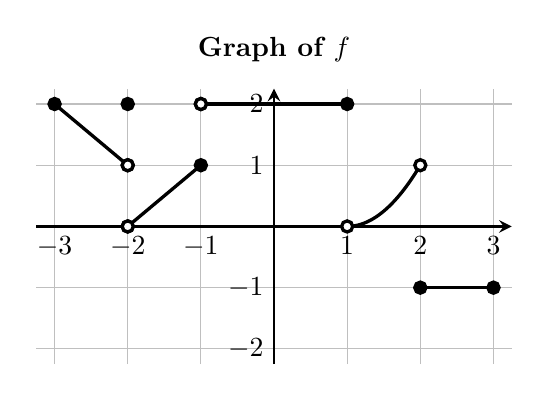
\begin{tikzpicture}
\begin{axis}[
   	xmin=-3.25, xmax=3.25,
	ymin=-2.25, ymax=2.25,
	major tick length={0},
	xtick={-3,-2,...,3}, ytick={-2,-1,...,2},
	line width=1pt, title={\textbf{Graph of $f$}},
 	axis lines=center, height=2 in, width=3 in, grid=major,
 	restrict y to domain=-2.25:2.25
	]
	\addplot [mark=*, black, smooth, very thick] plot coordinates {(-3,2)(-2,1)};
	\addplot [mark=*, black, smooth, very thick] plot coordinates {(-2,3)};
	\addplot [mark=*, black, smooth, very thick] plot coordinates {(-2,0)(-1,1)};
	\addplot [mark=*, black, smooth, very thick] plot coordinates {(-1,2)(1,2)};
	\addplot [mark=*, black, smooth, very thick] plot coordinates {(2,-1)(3,-1)};
    \addplot [black, smooth, very thick, samples=100, domain=1:2] {(x-1)^2};
    \addplot [black, only marks, very thick, mark=*, mark options={scale=1, fill=white}]
    coordinates{(1,0) (2,1) (-1,2) (-2,1) (-2,0)};
    \addplot [black, only marks, very thick, mark=*] coordinates{(-2,2)};
\end{axis}
\end{tikzpicture}
%\end{center}
}
\end{minipage}}

\newcommand{\ggraff}{
\begin{minipage}[l][.30\textwidth]{3 in}{
%\begin{center}
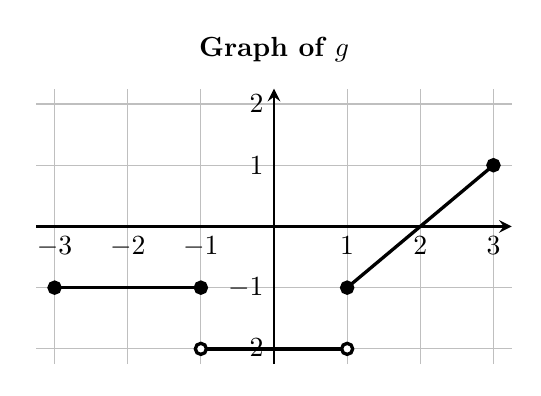
\begin{tikzpicture}
\begin{axis}[
   	xmin=-3.25, xmax=3.25,
	ymin=-2.25, ymax=2.25,
	major tick length={0},
	xtick={-3,-2,...,3}, ytick={-2,-1,...,2},
	line width=1pt, title={\textbf{Graph of $g$}},
 	axis lines=center, height=2 in, width=3 in, grid=major,
 	restrict y to domain=-2.25:2.25
	]
	\addplot [mark=*, black, smooth, very thick] plot coordinates {(-3,-1)(-1,-1)};
	\addplot [mark=*, black, smooth, very thick] plot coordinates {(1,-1)(3,1)};
	\addplot [black, very thick, mark=*, mark options={scale=1, fill=white}] plot coordinates {(-1,-2)(1,-2)};
\end{axis}
\end{tikzpicture}
%\end{center}
}
\end{minipage}}

\begin{document}
\begin{center}
\textbf{
    Sample problems with solutions for Homework 2}
\end{center}
    \begin{enumerate}
        \item Rewrite the following expression using summation notation:
        $\ln\left(\prod_{k=1}^4 x_k\right)$
        \item Find explicit formulas for a sequence with the following recursive rules.
        \begin{enumerate}
            \item $a_1 = 9$ and $a_n = 8a_{n-1}$ for $n \geq 2$

            \item $b_1 = 9$ and $b_n = 8nb_{n-1}$ for $n \geq 2$
        \end{enumerate}
        
        \item Each of the following sums is equal to exactly one of the others. Please find all of the pairs.
        \begin{enumerate}[label=(\alph*)]
            \item $\sum_{k=0}^{m+1} (3k+3)$
            \item $\sum_{k=1}^m (k+2)$
            \item $\sum_{k=2}^{m+3} (3k-5)$
            \item $\sum_{k=2}^{m+2} k$
            \item $\sum_{k=1}^{m+2} 3k$
            \item $\sum_{k=0}^{m} (k+2)$
            \item $\sum_{k=0}^{m+1} (3k+1)$
            \item $\sum_{k=0}^{m-1}(k+3)$
        \end{enumerate}
        \item Using the graphs below, find 
        \begin{enumerate}

            \item $\displaystyle \lim_{x\rightarrow 1^-} g(f(x))$
            \item $\lim_{x\rightarrow 1^+} g(f(x))$ 
            \item $\lim_{x\rightarrow 1^-} f(g(x))$
            \item $\lim_{x\rightarrow 1^+} f(g(x))$ 
                               \begin{center}
                    \begin{tabular}{l r}
                    \fgraff & \ggraff
                    \end{tabular}
                    \end{center}
        \end{enumerate}
    \end{enumerate}
    
    \newpage
    \begin{center}
        \textbf{\Large{Solutions}}
    \end{center}
    \begin{enumerate}
        \item Explicitly expanding the product notation to see the details fully fleshed out, we see:
        \begin{eqnarray*}
        \ln\left(\prod_{k=1}^4 x_k\right) &=& \ln(x_1\cdot x_2\cdot x_3\cdot x_4) \\[1em]
        &=& \ln(x_1) + \ln(x_2) + \ln(x_3) + \ln(x_4) \\[1em]
        &=& \sum_{k=1}^4 \ln(x_k)
        \end{eqnarray*}
        \item To find the pattern for the following, we write terms until we see a pattern arise.
        \begin{enumerate}
            \item  
            \begin{enumerate}[label=(\roman*)]
                \item $a_1=9$
                \item $a_2 = 8\cdot 9$
                \item $a_3=8\cdot (8\cdot 9)$
                \item $a_4= 8 \cdot (8\cdot 8\cdot 9)$
            \end{enumerate}
            From this, we can see we have one more 8 multiplied each step, and the 9 is just along for the ride.  Thus the general formula will be given by:
            \[a_n=9\cdot 8^{n-1}\]
            \item This one is similar, just a little more work:
            \begin{enumerate}
                \item $b_1=9$
                \item $b_2=8\cdot 2\cdot 9$
                \item $b_3=8\cdot 3\cdot (8\cdot 2\cdot 9)$
                \item $b_4=8\cdot 4 \cdot (8\cdot 3 \cdot 8 \cdot 2\cdot 9)$
                \item $b_5=8\cdot 5\cdot(8\cdot 4 \cdot 8\cdot 3 \cdot 8 \cdot 2\cdot 9)$
            \end{enumerate}
            If we look carefully, we can see a factorial pattern arise, as well as an accumulation of 8s.  There is also the extra 9 that is in each term.  Putting this together, we get:
            \[b_n=9\cdot n!\cdot 8^{n-1}\]
        \end{enumerate}
        \item To find which ones are equal, one could compute each sum (which would depend on $m$ or pick one and search through the others to find the match by comparing terms.  I prefer the latter, at least for such a small sampling of summations. 
        \begin{itemize}
            \item $(a)=(e)$
            \item $(b)=(h)$
            \item $(c)=(g)$
            \item $(d)=(f)$
        \end{itemize}
        \item 
        \begin{enumerate}
            \item To compute $\displaystyle \lim_{x\rightarrow 1^-} g(f(x))$, we start by examining the behavior of $f(x)$ as $x\rightarrow 1^-$. We see that $f(x)$ has a constant value of $2$. Substituting $x=2$ into $g(x)$ gives $0$, so $\displaystyle \lim_{x\rightarrow 1^-} g(f(x)) = 0$.
            \item For $\lim_{x\rightarrow 1^+} g(f(x))$, we similarly examine the behavior of $f(x)$, but this time as $x\rightarrow 1^+$. We find $\lim_{x\rightarrow 1^+} f(x) = 0$. But notice that the $y$-values of $f(x)$ are approaching $0$ from above, and thus decreasing towards 0. Since these are the values that are substituted into $g(x)$ we must find
            $\lim_{x\rightarrow 0^+}g(x)$, which gives $-2$.
            \item This time, for $\lim_{x\rightarrow 1^-} f(g(x))$, we examine the behavior of $g(x)$ as $x\rightarrow1^-$. We see $\lim_{x\rightarrow 1^-} g(x) = 2$. But notice that the $y$-values are a constant value of $2$. These are the values that are being substituted into $f(x)$, so rather than taking a limit of $f(x)$, we just need the value of $f(-2)$, which is $2$.
            \item For $\lim_{x\rightarrow 1^+} f(g(x))$, we first look at the behavior of $g(x)$ as $x\rightarrow 1^+$. We see this limit is $\lim_{x\rightarrow 1^+} g(x) = -1$. The $y$-values are approaching $-1$ from above, which means the values are decreasing towards $-1$. Substituting into $f(x)$, we see that we need $\lim_{x\rightarrow -1^+} f(x)$, which from the graph is 2.
        \end{enumerate}
    \end{enumerate}
\end{document}